% !TEX root = \linearpartition.tex


\subsection{Efficiency and Scalability}

We compare the efficiency of \linearpartition with the baseline \viennarnafold
(Version 2.4.11) (\url{https://www.tbi.univie.ac.at/RNA/download/sourcecode/2_ 4_x/ViennaRNA-2.4.11.tar.gz}).
\viennarnafold is a widely-used RNA structure prediction package,
and provides partition function and base pair probabilities calculation based on classical cubic runtime algorithm.
We use the ArchiveII dataset, % \cite{sloma+mathews:2016}, 
a comprehensive set of well-determined structures first curated in the 1990s 
\cite{mathews+:1999}% [72] 
and updated later with additional structures 
\cite{sloma+mathews:2016}% [96].  
(\url{http://rna.urmc.rochester.edu/pub/archiveII.tar.gz}; 
we removed those sequences found in the S-Processed set).
The dataset contains 2889 RNA sequences from 9 families, 
and the average length is 222 $nt$ and max length is 2968 $nt$.
We run all programs (compiled by GCC 4.9.0) on Linux, 
with 2.90GHz Intel Core i9-7920X CPU and 64G memory.

\begin{figure}[H]
\center
\includegraphics[scale=1.16]{figs/runtime_desktop_bpp_vienna_b2}
\caption{Runtime comparisons on thze ArchiveII dataset between with the baseline, \viennarnafold, and \linearpartition. 
The curve-fittings were done log-log in gnuplot with $n > 10^3$.
\label{runtime}}
\end{figure}

Figure~\ref{runtime} confirms that runtime of \linearpartition scales linearly with sequence length, while the baseline \viennarnafold scale cubically. For a sequence of 2,968 $nt$ (23S rRNA), \linearpartition takes only 7 seconds while the baselines take 75 seconds. This clearly shows the advantage of \linearpartition on very long ncRNAs.


\subsection{Accuracy}

\begin{figure*}[t]
\center
\begin{tabular}{cc}
\panel{A} & \panel{B} \\[-0.5cm]
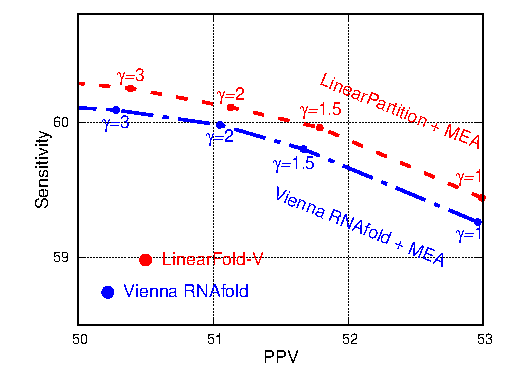
\includegraphics[scale=.7]{figs/new_MEA_diff_gamma_beam_inf_threshold_001}
&
\raisebox{-0.25cm}{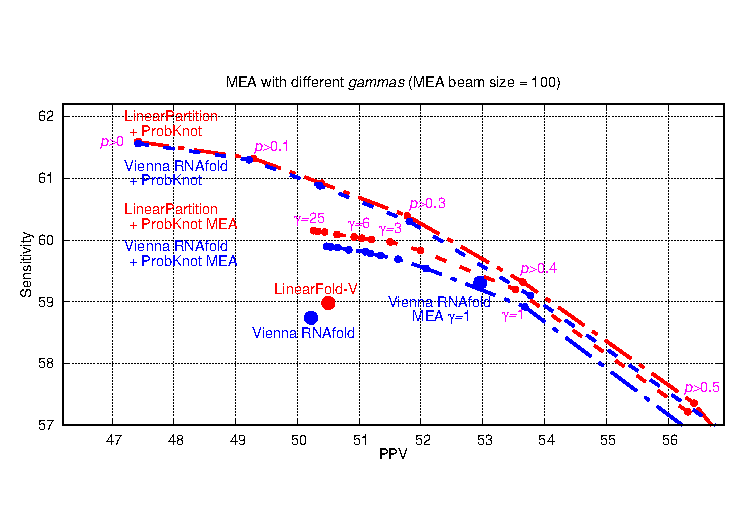
\includegraphics[scale=.58]{figs/MEA_gamma_B100}}

\end{tabular} % A: specify MFE in label
\caption{Accuracy comparison for two systems.
	{\bf A}: Overall MFE and MEA structure PPV-sensitivity tradeoff of two systems with varying $gamma$. 
	{\bf B}: Overall ThreshKnot structure PPV-sensitivity tradeoff of two systems with varying $gamma$
	% {\bf C}:
	\linearpartition even leads to a small improvement in the downstream MEA predictoin using the probability matrix computed in linear time.
	\label{mea}
}
\end{figure*}

\iffalse
\begin{figure*}[t]
\center
\begin{tabular}{ccc}
\hspace{-0.5cm}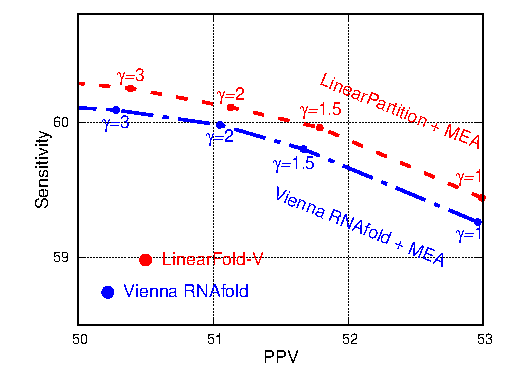
\includegraphics[scale=.8]{figs/new_MEA_diff_gamma_beam_inf_threshold_001}
&
\hspace{-1.85cm}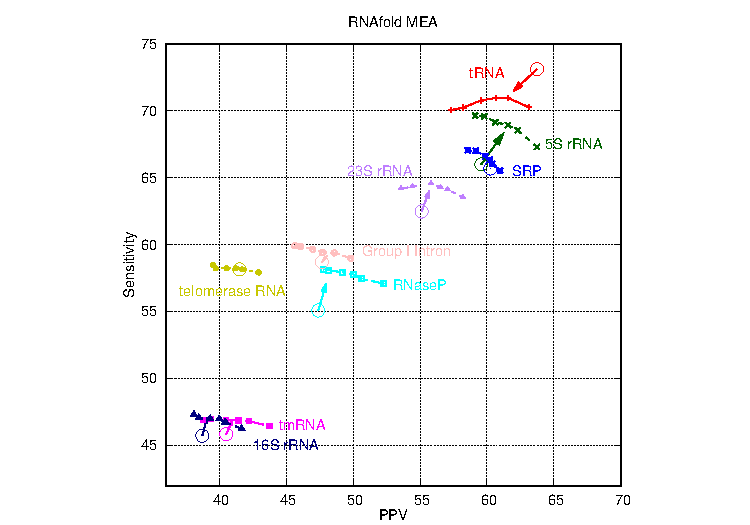
\includegraphics[scale=.58]{figs/new_MEA_RNAfold_diff_gamma_families}
&
\hspace{-2.35cm}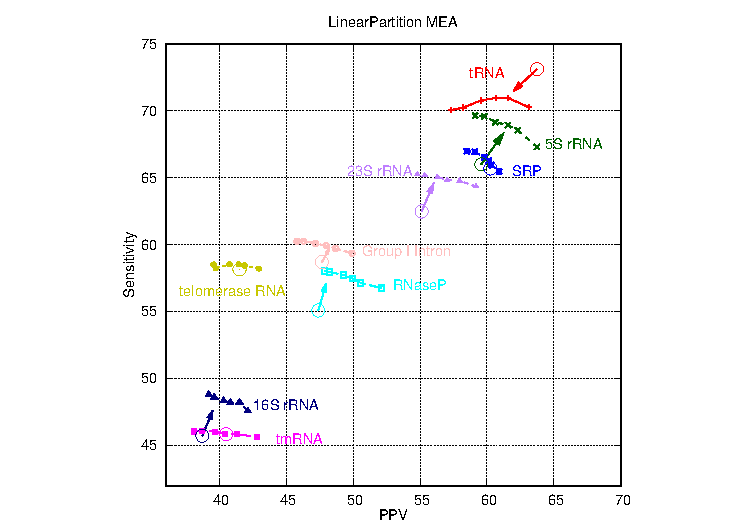
\includegraphics[scale=.58]{figs/new_MEA_LinearPartition_diff_gamma_families}

\end{tabular} % A: specify MFE in label
\caption{MFE and MEA structure accuracy comparison for two systems.
	{\bf A}: Overall PPV-sensitivity tradeoff of two systems with varying $gamma$. 
	{\bf B}:
	{\bf C}:
	\linearpartition even leads to a small improvement in the downstream MEA predictoin using the probability matrix computed in linear time.
	\label{mea}
}
\end{figure*}
\fi

We next compare accuracy of \linearpartition with the baseline \viennarnafold.
We take the base pair probability matrices from these two systems, 
and fed them to standard MEA algorithm.
We use Positive Predictive Value (PPV, the fraction of predicted pairs in the known structure) and sensitivity (the fraction of known pairs predicted) to measure the accuracy across all families, as well as slipping method to allow base pair to slip by one nucleotide \cite{sloma+mathews:2016}.


% Figure~\ref{mea} shows that \linearpartition even leads to a small improvement in the downstream MEA predictoin using the probability matrix computed in linear time. 
% Figure~\ref{mea} gives the accuracy comparison between 
Figure~\ref{mea}A shows that 
(1) MEA-based method is more accurate than MFE-based method for both systems; 
(2) \linearpartition + MEA is constantly more accurate than \viennarnafold + MEA.
With the same $\gamma$, a hyperparameter balances PPV and sensitivity in MEA algorithm,
\linearpartition + MEA enjoys a small improvement in both PPV and sensitivity.


% ThreshKnot
Probknot is another partition-function-based method which is much simpler than MEA, only adds a linear post-processing step after the partition function calculation, and can predict pseudoknots. 
Recently, ThreshKnot \cite{Liang+:2019}, a simple thresholded version of ProbKnot, 
leads to more accurate overall predictions by filtering out unlikely pairs whose prob falls under a given threshold,
so we also compare ThreshKnot structure accuracy.

Figure~\ref{mea}B shows that ???????

per family accuracy

% Figure 3B shows that LinearFold is more accurate than the baselines, and interestingly, this advantage is more pronunced on longer sequences, esp. the two longest families in the database, 16S and 23S Ribosomal RNAs.

\iffalse
\begin{figure}[H]
\center
\begin{tabular}{cc}
\multicolumn{2}{c}{\hspace{-1cm}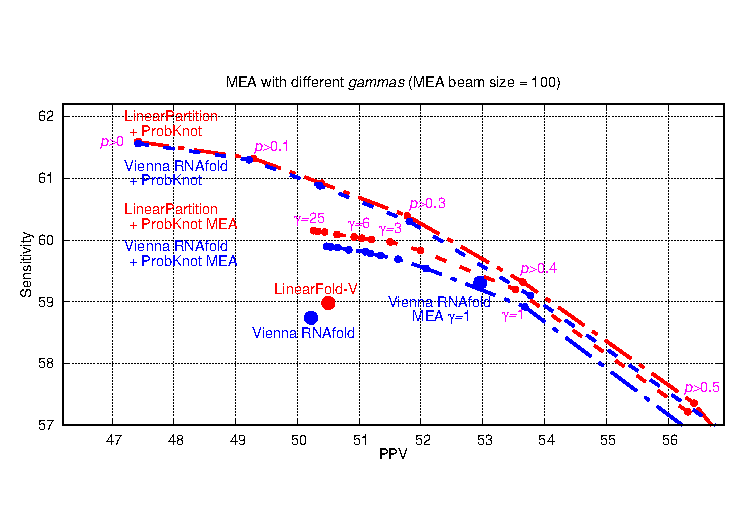
\includegraphics[scale=.7]{figs/MEA_gamma_B100}}
\\
\hspace{-0.5cm}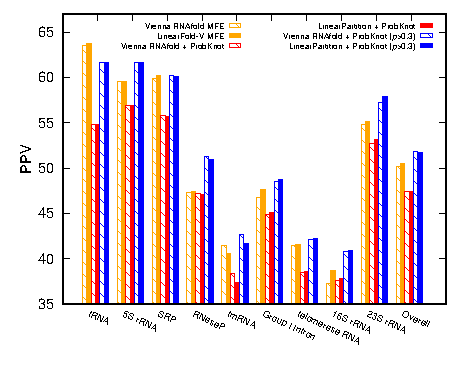
\includegraphics[scale=.68]{figs/ProbKnot_PPV}
&\hspace{-0.5cm}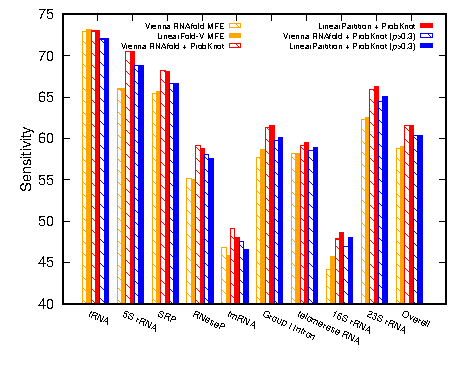
\includegraphics[scale=.68]{figs/ProbKnot_Sens}
\end{tabular}
\caption{ThreshKnot structure accuracy comparison.
	{\bf A}
	{\bf B}
	{\bf C}
	\label{probknot}
}
\end{figure}
\fi



\subsection{Search Quality}

Fig. 4A–B show that our \linearpartition algorithm can indeed approximate the partition function reasonably well. 
Here we measure root-mean-square deviation (RMSD) between the two probability matrices $p$ and $p'$ (from Vienna RNAfold and \linearpartition, resp.) 
over the set of all possible pairs pairs($x$) on a sequence $x$ (i.e., ${\rm{pairs}}(x)={1\leq{i}<j\leq{|x|} \ | \  x_{i}x_{j} \in {\rm CG, GC, AU, UA, GU, 
UG},j-i>3}$): 

\begin{equation}
{\rm{RMSD}}(p,p')=\sqrt{\frac{1}{|{\rm{pairs}}(x)|}\sum_{(i,j) \in {{\rm{pairs}}(x)}}{(p_{i,j}-p'_{i,j})}^2}
\end{equation}

\begin{figure*}[t]
\center
\begin{tabular}{cc}
\panel{A} & \panel{B} \\[-0.4cm]
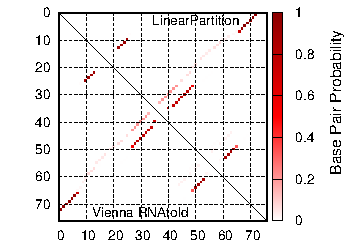
\includegraphics[width=0.3\textwidth]{figs/tRNA_identical_heatmap}
&
{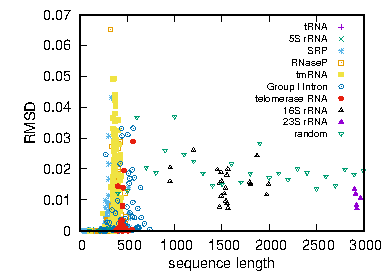
\includegraphics[width=0.38\textwidth]{figs/rmsd_family_plus_random_b2}}
\\[-0.2cm]
\panel{C} & \panel{D}\\[-0.5cm]
\hspace{-0.5cm}\raisebox{-0.45cm}{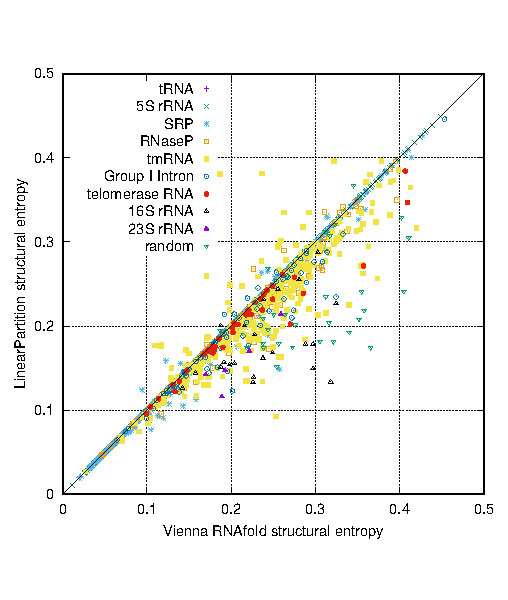
\includegraphics[width=0.28\textwidth]{figs/structure_entropy_xy_plus_random}}
&
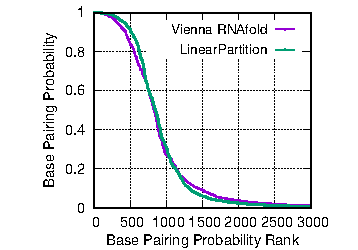
\includegraphics[width=0.38\textwidth]{figs/sorted_prob_23s}
\end{tabular}
\caption{
Comparison of base pair probabilities from \viennarnafold and \linearpartition.
	{\bf A}: \linearpartition (upper triangle) and Vienna RNAfold (lower triangle) result in identical base pair probability matrix for {\it E.~coli} tRNA$^\textit{Gly}$.
	{\bf B}: root-mean-square deviation (RMSD) is relatively small between \linearpartition and Vienna RNAfold.
	{\bf C}: structural entropy comparison.
	{\bf D}: \linearpartition starts higher and finishes lower than RNAfold in a sorted probability curve for \ecoli 23S rRNA.
	\label{sq}
}
\end{figure*}

Figure~\ref{sq}A shows the probability matrix for short sequence, e.g. tRNA sequence, from both RNAfold and \linearpartition yield identical matrices (i.e., RMSD=0). Figure~\ref{sq}B shows that RMSD is relatively small across all RNA families in the ArchiveII dataset. The highest deviation is 0.067 for one RNaseP sequence, which means on average, each pair’s probability deviation in that worst-case sequence is about 0.067 between the exact algorithm and our linear-time one. With sequence length increasing, RMSD gradually decreases, since the number of possible pairs grows in $O(n^2)$ but the number of highly probable pairs grows in $O(n)$; on the longest 23S rRNA family, RMSD is about 0.015. We also included 30 random RNA sequences with length 100–3,000 and they behave similarly to natural sequences in terms of RMSD. 

% Figure~\ref{sq}C and D show
We assume \linearpartition base pair probability distribution is peakier since it ignores low energy substructure in partition function calculation.
We uses structural entropy \cite{Huynen+:1997} to measure this, 
where lower structural entropy indicates that the distribution is dominated by fewer base pairing probabilities.
Figure~\ref{sq}C shows \linearpartition distribution is peakier (lower structural entropy) than RNAfold for most sequences.

We also uses \ecoli 23S rRNA as an example to illustrate the distribution difference.
We sort all base pair probabilities from high to low and take the top 3,000 rank.
Figure~\ref{sq}D shows \linearpartition probability distribution curve starts higher and finishes lower.


\subsection{Beam Size Impact}



\begin{figure}[H]
\center
\includegraphics[width=0.48\textwidth]{figs/RMSD_beamsize}
\end{figure}

\subsection{Example}


